\documentclass{article}
\usepackage[utf8]{inputenc}
\usepackage{amsfonts}
\usepackage{algorithm2e}
\usepackage{amsmath}
\usepackage[a4paper]{geometry}
\geometry{hscale=0.8,vscale=0.9,centering}
\usepackage{graphicx}
\usepackage{program}
\usepackage{ulem}
\usepackage{xcolor}
\usepackage{pdfpages}
\usepackage{hyperref}
\newcommand{\subsubsubsection}[1]{\paragraph{#1}\mbox{}\\}
\setcounter{secnumdepth}{4}
\setcounter{tocdepth}{4}
\newcommand{\alinea}{
\textbf{\hspace{8mm}}
}
 \setlength{\parindent}{0pt}
 
\newcommand{\sautligne}{
\textbf{\vspace{5mm}}
}
\usepackage{pdflscape}
\newenvironment{changemargin}[2]{%
\begin{list}{}{%
\setlength{\topsep}{0pt}%
\setlength{\leftmargin}{#1}%
\setlength{\rightmargin}{#2}%
\setlength{\listparindent}{\parindent}%
\setlength{\itemindent}{\parindent}%
\setlength{\parsep}{\parskip}%
}%
\item[]}{\end{list}}


\title{M1 Info – ARC - LAB4}
\author{Olivier HUREAU - Groupe 3}
\date{06/04/2020}

\begin{document}
\maketitle
\renewcommand{\contentsname}{Table des matières}
\tableofcontents
\newpage

\section{Évaluation de la qualité des tests.}
Les différents types de couverture nous intéréssant sont 
\begin{itemize}
	\item State / Transition coverage : En principe les testbench vérifie que la machine passe dans tout les états. Si nous n'avons pas 100\% de couverture ici c'est qu'il y a un problème.
		\item Branch coverage : Si le teste de couverture remonte des erreurs, il sera alors plus facile de traquer les erreurs de transissions..
	\item Statement coverage : Les statements influant sur les branchements, ce test de couverture nous permet aussi de vérifier le comportement du robot.

\end{itemize}

Les tests "line coverage"  donnent une indication sur la présentation ou l'optimisation du code, ne nous souciant uniquement du bon fonctionnement de notre implémentation, il ne nous sont pas utile.

Le test Toggle coverage donnant une indication sur la robustesse du l'implémentation. Il est bien trop compliqué et trop long d'analyser les résultats de ce test dans le cadre de nos labs.


\subsection{Première analyse}

\subsubsection{Résultats du test de coverage}

\paragraph{Résultats du test de coverage sur le système entier}

Ci dessous : S est l'architecture System, C1 et C2 les compteurs et R le robot dans le testbench System.
\begin{figure}[!h]
\advance\leftskip+3cm
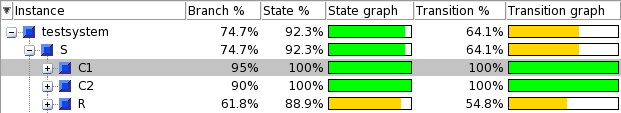
\includegraphics[scale=0.70]{PremiereAnalyse/Coverage.PNG}
\caption{Résultats de couverture Branch, State et Transition sur le système entier}
\end{figure}

Le graph de couverture du robot dans le testbench system

\begin{figure}[!h]
\advance\leftskip+3cm
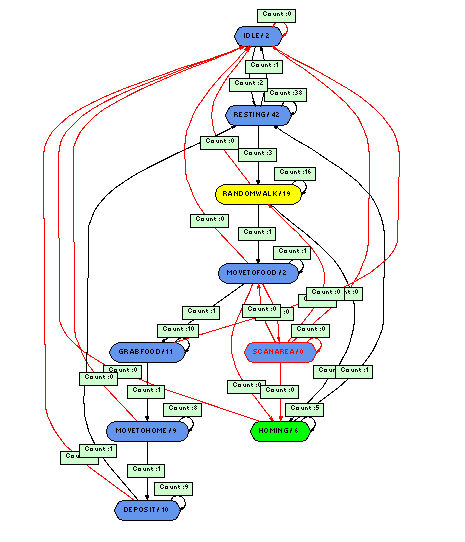
\includegraphics[scale=0.80]{PremiereAnalyse/graph.PNG}
\caption{Graph de couverture d'état sur le système entier}
\end{figure}

\paragraph{Résultats du test de coverage sur le robot}

Ci dessous : S est l'architecture System, C1 et C2 les compteurs et R le robots dans le testbench System.
\begin{figure}[!h]
\advance\leftskip+3cm
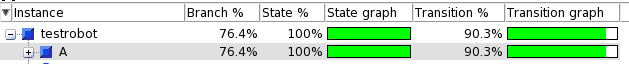
\includegraphics[scale=0.70]{PremiereAnalyse/coverRobot.PNG}
\caption{Résultats de couverture Branch, State et Transition sur le robot}
\end{figure}

Le graph de couverture du robot dans le testbench system

\begin{figure}[!h]
\advance\leftskip+3cm
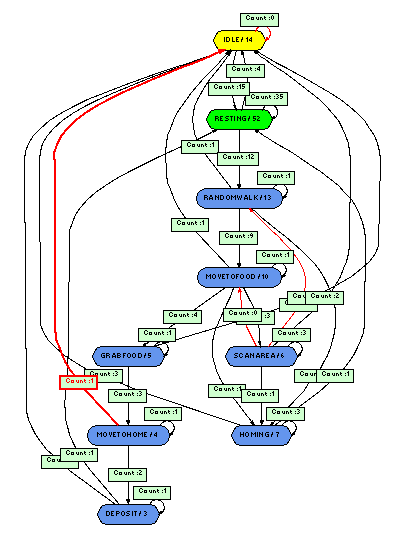
\includegraphics[scale=0.65]{PremiereAnalyse/graphRobot.PNG}
\caption{Graph de couverture d'état sur le robot}
\label{graphe-robot}
\end{figure}.



On observera aussi le code coverage analysis :

\begin{figure}[!h]
\advance\leftskip+3cm
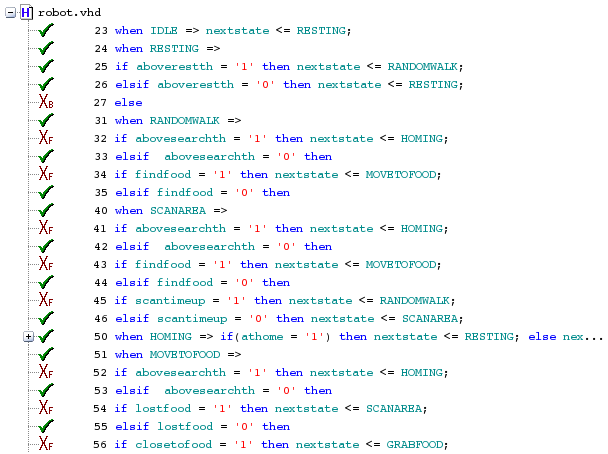
\includegraphics[scale=0.7]{PremiereAnalyse/codeCov.PNG}
\caption{Graph de couverture d'état sur le robot}

\end{figure}


\paragraph{Interprétation des résultats}
Les tests de couverture sont très probant (78.5\% pour le système entier). Cependant, on vois que des dans le système entier, l'état SCANAREA n'est jamais atteins bien que les tests de système (se reporter au tableau du précédent lab) avaient prévu un chemin pour arriver jusqu'à cet état ainsi que l'utilisation de ses transitions. 

L'analyse du robot avec un testbench différent nous donne alors des indications suivantes : certaines transitions ne sont jamais atteintes, l'état SCANAREA est bien accessible pour l'automate. 
\sautligne

Deux hypothèses se posent alors : Soit le système est mal conçus, soit c'est les testbenchs. Avant de se replonger dans une éventuelle réécriture des architectures et/ou entitées (la couverture des branch pourrons nous aider pour cela). Il faut être certains que les testbenchs sont correct.

Après interprétation des résultats, on créera des séquences de signaux qui nous permettrons d'être sur que le testbenchs du robot n'est pas faux.



\subsection{Correction du code après une première analyse }

\subsubsection{Correction du testbench du robot}

\paragraph{Les branchements}

Le code coverage analysis nous indique que certains branchements ne sont pas exécuté. En effet, j'avais mis des sécurités sur mes conditions. Prennons l'exemple suivant : .

\begin{verbatim}
if aboverestth = '1' then nextstate <= RANDOMWALK;
elsif aboverestth = '0' then nextstate <= RESTING;
\end{verbatim} 

Je voulais être sur que le deuxième statement ne s'execute uniquement si aboverestth vaut '0' et non pas si aboverestth est différent de '1', étant donné la structure std\_logic

Je ne sais pas si je dois garder cette sécurité.. Pour les tests de couverture, je l'enlève donc.

\sautligne

\paragraph{Les etats et les transitions}
Grace au graph de couverture (figure \ref{graphe-robot}) il faut tester les transitions suivantes :
\begin{itemize}
\item Reset depuis MOVETOHOME
\item Aller de SCANAREA à MOVETOFOOD (rappel de contraintes de transition : Aboveseartch ='0' \& findfood = '0' \& scantimeup = '1')
\item Aller de SCANAREA à RANDOMWALK (rappel de contraintes de transition : Aboveseartch ='0' \& findfood = '1' )
\end{itemize}

\paragraph{Résultat après correction}
Après correction, on obtiens donc les résultats suivants :

\begin{verbatim}
Coverage Report Summary Data by file

=================================================================================
=== File: /tp/xm1iarc/xm1iarc003/projet_asic/ARC/lab4/robot.vhd
=================================================================================
    Enabled Coverage            Active      Hits    Misses % Covered
    ----------------            ------      ----    ------ ---------
    Stmts                           28        28         0     100.0
    Branches                        43        43         0     100.0
    FEC Condition Terms             11        11         0     100.0
    FSMs                                                       100.0
        States                       9         9         0     100.0
        Transitions                 31        31         0     100.0

=================================================================================
=== File: /tp/xm1iarc/xm1iarc003/projet_asic/ARC/lab4/testRobot.vhd
=================================================================================
    Enabled Coverage            Active      Hits    Misses % Covered
    ----------------            ------      ----    ------ ---------
    Stmts                           14        14         0     100.0


Total Coverage By File (code coverage only, filtered view): 100.0%
\end{verbatim}

\begin{figure}[!h]
\advance\leftskip+3cm
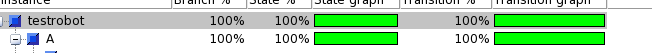
\includegraphics[scale=0.7]{PremiereCorrection/resultats.PNG}
\caption{Rapport de couverture}

\end{figure}

\paragraph{Conclusion de la correction du robot}
Avec ces tests de couvertures qui sont concluant, on peux donc affirmer que le robot se comporte correctement grâce au modifications effectué sur notre code.

Voir annexes : 

\subsubsection{Correction du testbench du system}

On sait ici que plusieurs problèmes sont à résoudre pour obtenir un test de couverture concluant. Il faut donc : 
\begin{itemize}
\item Passer dans l'état SCANAREA
\item Utiliser les différentes transitions :
	\begin{itemize}
	\item MOVETOFOOD vers SCANAREA (Contraines : abovesearchth = '0' \& losftood = '1' )
	\item SCANAREA vers RANDOMWALK (Contraines: abovesearchth = '0' \& findfood = '0' \& scantimeup = '1'  )
	\item SCANAREA vers MOVETOFOOD (Contraines : abovesearchth = '0' \& findfood = '1' )
	\item SCANAREA vers HOMING (Contraines : abovesearchth ='1' )
	\end{itemize}
\item Utiliser le reset pour tout les états
\end{itemize}

\paragraph{Résultat après correction}
Après correction, on obtiens donc les résultats suivants :
\begin{verbatim}
Coverage Report Summary Data by file

=================================================================================
=== File: /tp/xm1iarc/xm1iarc003/projet_asic/ARC/lab4/count.vhd
=================================================================================
    Enabled Coverage            Active      Hits    Misses % Covered
    ----------------            ------      ----    ------ ---------
    Stmts                           17        17         0     100.0
    Branches                        20        19         1      95.0
    FEC Condition Terms             10         6         4      60.0
    FSMs                                                       100.0
        States                       2         2         0     100.0
        Transitions                  4         4         0     100.0

=================================================================================
=== File: /tp/xm1iarc/xm1iarc003/projet_asic/ARC/lab4/robot.vhd
=================================================================================
    Enabled Coverage            Active      Hits    Misses % Covered
    ----------------            ------      ----    ------ ---------
    Stmts                           28        28         0     100.0
    Branches                        43        43         0     100.0
    FEC Condition Terms             11        11         0     100.0
    FSMs                                                        87.0
        States                       9         9         0     100.0
        Transitions                 31        23         8      74.1

=================================================================================
=== File: /tp/xm1iarc/xm1iarc003/projet_asic/ARC/lab4/testSystep.vhd
=================================================================================
    Enabled Coverage            Active      Hits    Misses % Covered
    ----------------            ------      ----    ------ ---------
    Stmts                           12        12         0     100.0


Total Coverage By File (code coverage only, filtered view): 91.9%

\end{verbatim}



\begin{figure}[!h]
\advance\leftskip+0cm
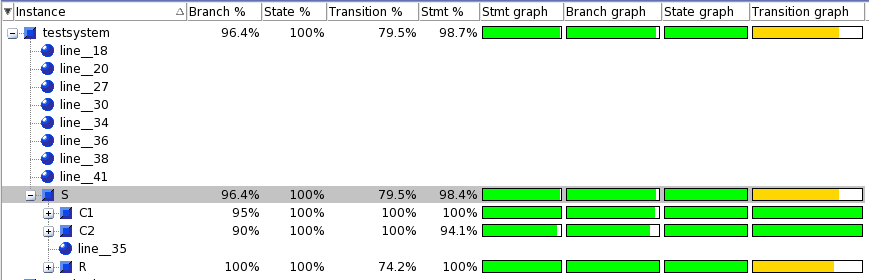
\includegraphics[scale=0.7]{PremiereCorrection/ResAfterVHD.PNG}
\caption{Rapport de couverture}

\end{figure}

\begin{figure}[!h]
\advance\leftskip+3cm
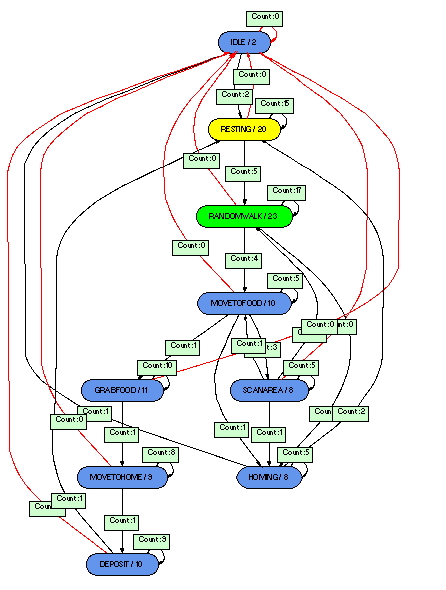
\includegraphics[scale=0.7]{PremiereCorrection/GRAPH.PNG}
\caption{Graph de couverture des états du robot}

\end{figure}


\paragraph{Interprétation des résultats}

La couverture n'est pas totales car je n'ai pas testé si le reset marche pour tout les états. De plus, les counters ne rentre pas dans les configurations permettant d'avoir un branching parfait sur ces éléments. 
\sautligne 

Néanmoins, je ne pense pas qu'il est nécessaire d'aller plus loin. Les tests de couvertures sont passé haut la main avec un Total Coverage by file the 91,9\%.

\newpage


\begin{landscape}
\section{Vérification d'assertions temporelles}

Ici, le code de P1 et P2 est faux, il est corrigé en section 4. La démonstration que l'assertion est juste reste néanmoins la même.

\subsection{P1}
\uline{Chaque fois que le robot commence sa recherche, il ne pourra pas atteindre l'état 
grabfood tant qu'il n'aura pas trouvé de nourriture (entrée findfood)}

\subsubsection{Formule PSL }
\begin{figure}[!h]
\centering
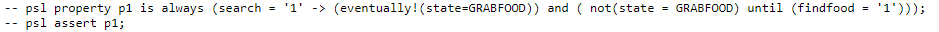
\includegraphics[scale=0.8]{PSL/P1.PNG}
\caption{PSL property P1}
\end{figure}

\subsubsection{Analyse du chronograme}
Dans un premier temps, on veux vérifier que l'assertion démarre lorsque search vaux 1. (Entouré en bleu ci dessous). 
En suite, on veux vérifier que l'assertion se finisse avec succès lorsqu'avant de passer dans l'état grabfood on détecte une findfood = '1' (entouré en rouge)

\begin{figure}[!h]
\advance\leftskip+0cm
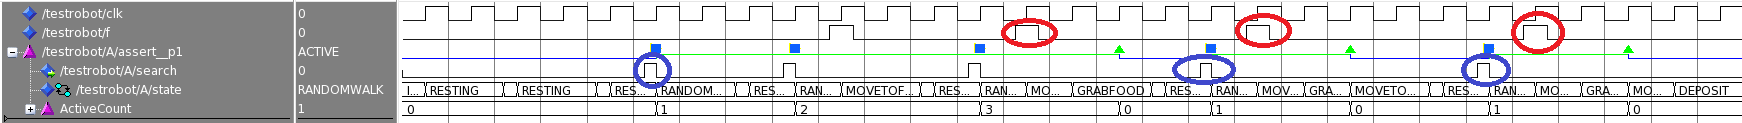
\includegraphics[scale=0.45]{PSL/P1-1.PNG}
\caption{Assertion P1 sur le chronograme }
\end{figure}

On vois alors bien ici que l'assertion se déclenche au bon moment et se termine avec succès comme souhaité.
 
\newpage
\subsection{P2}
\uline{Chaque fois que le robot commence sa recherche, il ne pourra pas atteindre l'état
homing tant qu'il n'aura pas dépassé le seuil du temps de recherche}
\subsubsection{Formule PSL }
\begin{figure}[!h]
\advance\leftskip+0cm
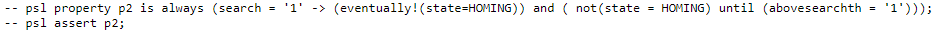
\includegraphics[scale=0.7]{PSL/P2.PNG}
\caption{PSL property P2}
\end{figure}

\subsubsection{Analyse du chronograme}


Ici on veux vérifier que l'assertion démarre en même temps que la recherche (losange roge), qu'aboveresearchth soit bien à '1' (rond rouge) avant de rentrer dans l'état homing (rectangle bleu).

\begin{figure}[!h]
\advance\leftskip+0cm
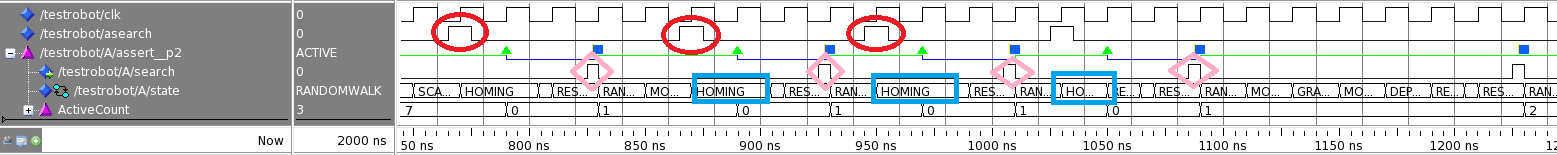
\includegraphics[scale=0.5]{PSL/P2-1.PNG}
\caption{Assertion P2 sur le chronograme }
\end{figure}

Tout ce passe comme prévu, la PSL property vérifie bien le comportement énoncé.

\newpage
\subsection{P3}
\uline{Chaque fois que le robot ramène de la nourriture, il devra passer par l'état deposit
avant de positionner la sortie rest à '1'
}






\subsubsection{Formule PSL }
\begin{figure}[!h]
\advance\leftskip+0cm
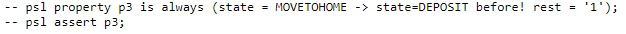
\includegraphics[scale=0.7]{PSL/P3.PNG}
\caption{PSL property P3}
\end{figure}

\subsubsection{Analyse du chronograme}
J'interprète ici le fait que le robot ramène de la nouriture lorsque qu'il rentre dans l'état MOVETOHOME.
\sautligne

Ce qui est intéréssant ici est que lorsqu'on fais un reset lors de la transition de IDLE à RESTING, on met aussi en sortie rest à 1. 



Il faut donc vérifier que :

\begin{itemize}
\item  L'assertion se déclenche bien à l'entrée de MOVETOHOME (rectangle bleu)
\item L'assertion s'arrête avec succès lorsque l'on rentre dans l'état déposit (rectangle vert)
\item L'assertion s'arrête avec un échec lorsqu'on effectue un reset (rond rouge)
\end{itemize} 


\begin{figure}[!h]
\advance\leftskip+0cm
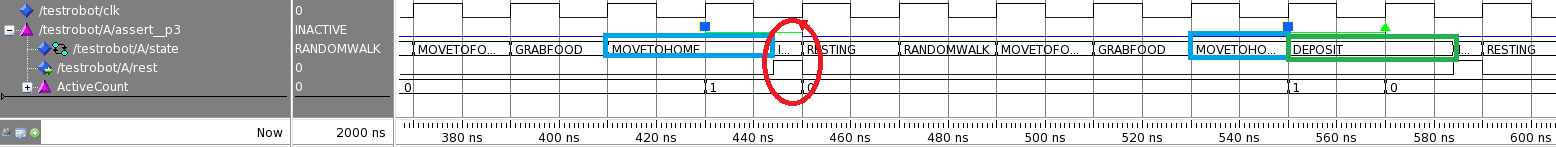
\includegraphics[scale=0.5]{PSL/P3-1.PNG}
\caption{Assertion P3 sur le chronograme }
\end{figure}


Les résultats sont concluants, la PSL property vérifie bien le comportement énoncé.

\newpage

\subsection{P4}
\uline{A partir du moment où le robot commence sa recherche, si abovesearchth n'est pas
atteint et qu'il trouve de la nourriture puis la perd puis il a dépassé le délai pendant lequel
il pouvait tenter à nouveau de l'approcher, alors il repasse dans l'état de recherche.}
\subsubsection{Formule PSL }
\begin{figure}[!h]
\advance\leftskip+0cm
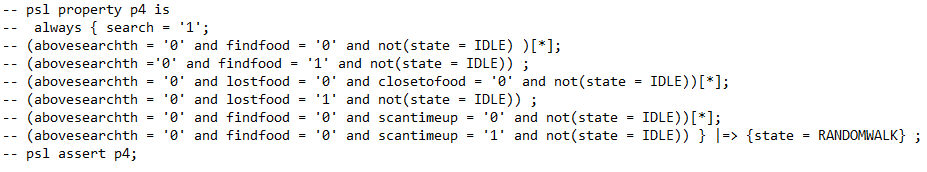
\includegraphics[scale=0.4]{PSL/P4.PNG}
\caption{PSL property P4}
\end{figure}

Pour cette propriété, j'ai jugé bon de rajouter le not(state = IDLE) car sinon la lecture des assertions n'était pas cohérente. Cela permet alors que l'assertion ne reste pas valide lors d'un reset. 

\alinea 

De plus, j'ai rajouté une contrainte closetofood ='0' par rapport à l'énoncé du tp pour éviter que lorsque le robot prend la transition de MOVETOFOOD vers GRABFOOD, l'assertion reste valide.
\sautligne

De plus, je me posais la question si ça devais être l'état RANDOMWALK ou le passage de rest à '1' qui déclenche l'assertion. Après quelques tests, si c'est l'état RANDOMWALK, alors plusieurs assertions peuvent se déclencher en même temps. C'est donc rest = '1' qui déclenchera l'assertion.

On obtiendras alors le chronograme ci dessous. 

\begin{figure}[!h]
\advance\leftskip+0cm
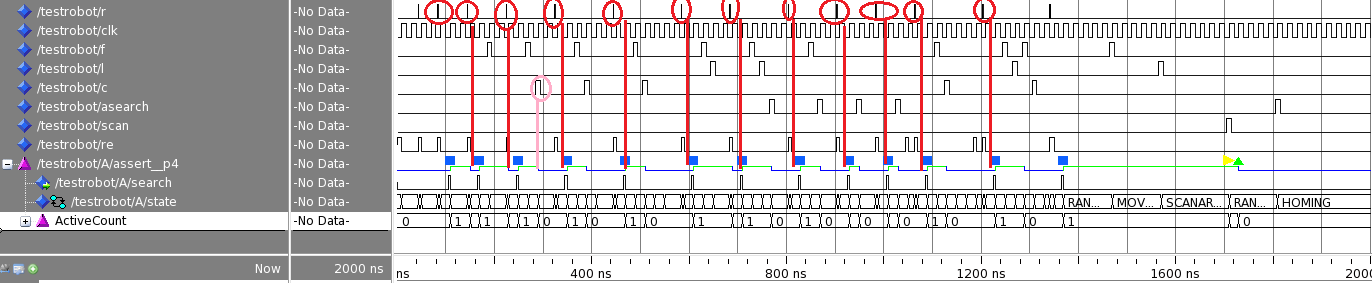
\includegraphics[scale=0.45]{PSL/P4-1.PNG}
\caption{Assertion P4 sur le chronograme }
\end{figure}

\newpage

Comme on ne s'intéresse pas aux assertions avec reset (rond rouge) et que le rond rose représente le chemin où closetofood = '1', je zoom donc sur la seul partie qui : nous intéresse.

On peux alors apercevoir les différents morceau de la phrase qui fait la description de l'assertion tel que :
\begin{itemize}
\item Label A : Chaque fois que le robot commence sa recherche
\item Label B : Puis abovesearchth n'est pasatteint et la nourriture n'est pas trouvée (pendant un nombre quelconque de cycles)
\item Label C : Puis abovesearchth n'est pas atteint et la nourriture est trouvée
\item Label D : Puis abovesearchth n'est pas atteint et lanourriture n'est pas perdue (pendant un nombre quelconque de cycles)
\item Label E : Puis abovesearchth n'est pas atteint et la nourriture est perdue
\item Label F : Puis abovesearchth n'est pas atteint et la nourriture n'est pas trouvée et le délai de récupération n'est pas dépassé i.e., scantimeup n'est pas à '1' (pendant un
nombre quelconque de cycles)

\item Label G :  Puis abovesearchth n'est pas atteint et la nourriture n'est pas trouvée
et le délai est dépassé 

\item Label H : Alors il doit repasser dans l'état de recherche


\end{itemize}

\begin{figure}[!h]
\advance\leftskip+0cm
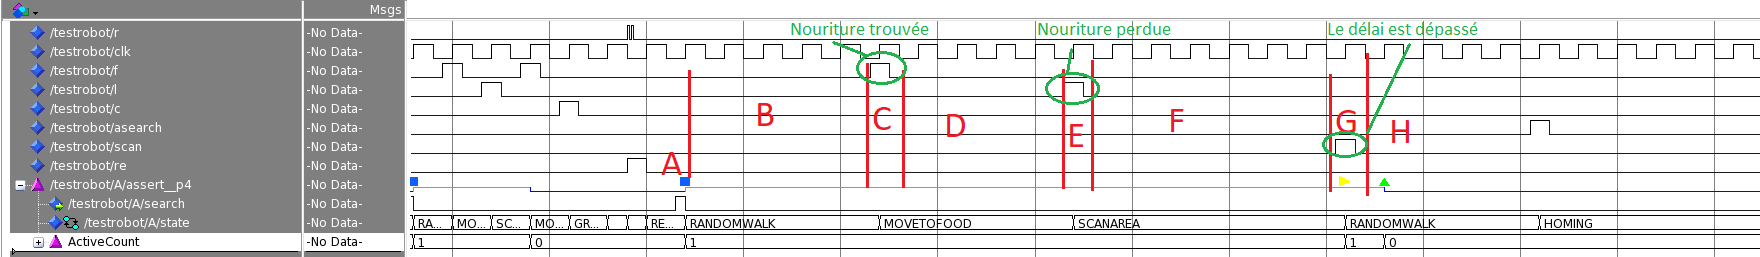
\includegraphics[scale=0.56]{PSL/P4-2.PNG}
\caption{Assertion P4 sur le chronograme }
\end{figure}

Les résultats sont concluants, la PSL property vérifie bien le comportement énoncé une première fois mais une assertion suivante n'est pas levé. J'avais donc tord. Il faut bien que ce soit l'état RANDOMWALK qui déclenche l'assertion. 

\newpage
\end{landscape}

Cependant,toutes les assertions se terminent quand abovesearch vaux '1' mais une assertion se lève aussi pendant le début de ce cycle et ne verras pas le signal d'arrêt :


\begin{figure}[!h]
\centering
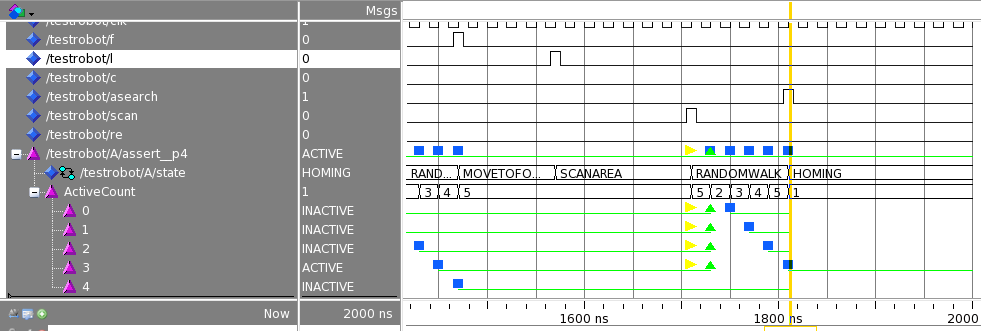
\includegraphics[scale=0.5]{PSL/P4-3.PNG}
\caption{Assertion P4 sur le chronograme }
\end{figure}

Pour régler le problème il faut vérifier que la première expréssion régulière vérifie que aboveresearchth soit bien à '0'.

On obtiens alors le chronograme suivant : 

\begin{figure}[!h]
\advance\leftskip+0cm
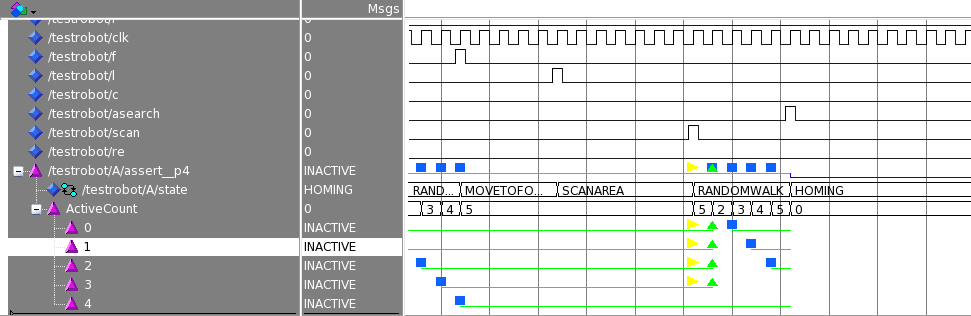
\includegraphics[scale=0.45]{PSL/P4-4.PNG}
\caption{Assertion P4 sur le chronograme }
\end{figure}

C'est bien ce que l'on attend.
\sautligne

Le code final de cette assertion est alors : 

 \begin{figure}[!h]
\advance\leftskip+0cm
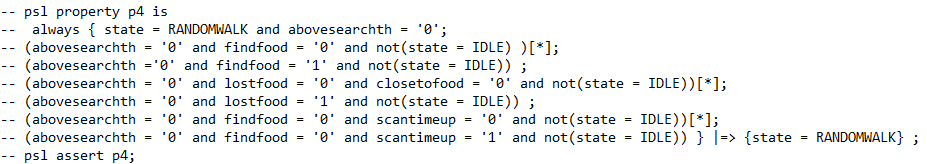
\includegraphics[scale=0.6]{PSL/P4-5.PNG}
\caption{Code final de P4 }
\end{figure}


\newpage
\subsection{P5}
\uline{Chaque fois que le robot est en phase de repos, il repassera inévitablement dans l'état
randomwalk.}
\subsubsection{Formule PSL }
\begin{figure}[!h]
\advance\leftskip+0cm
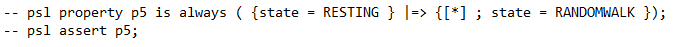
\includegraphics[scale=0.7]{PSL/P5.PNG}
\caption{PSL property P5}
\end{figure}

\subsubsection{Analyse du chronograme}

Comme précédement, on regarde quand est-ce que ça se déclenche et quand est-ce que ça s'arrête en succès.

\begin{figure}[!h]
\advance\leftskip+0cm
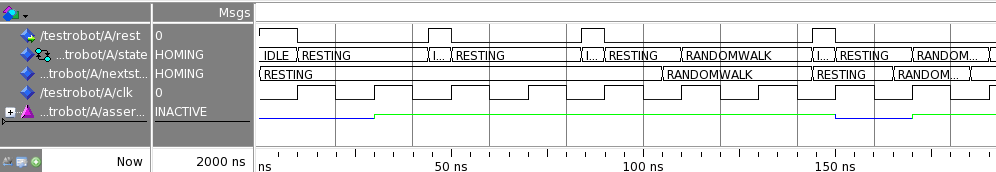
\includegraphics[scale=0.6]{PSL/P5-1.PNG}
\caption{Assertion P5 sur le chronograme }
\end{figure}

\subsubsection{ Réaliser une simulation
dans laquelle la condition attendue ne se produit pas}

Il suffit de faire de ne jamais mettre aboverestth à '1' dans le testbench.


\paragraph{Qu'observez-vous ?}

\sautligne

L'assertion reste valide tout le temps.

\paragraph{Que se passe-t-il
si vous faites alors "End simulation" dans ModelSim ?}

\sautligne

Une fenêtre nous demande si l'on est sur de bien vouloir quitter la simulation puis il est écris en sur la sortie stdout : 
\begin{verbatim}
# End time: 20:52:45 on Apr 05,2020, Elapsed time: 0:13:14
# Errors: 21, Warnings: 0
\end{verbatim}

\paragraph{ Comment interprétez-vous ce qui se
produit ?}


\sautligne

Que je ne pense pas qu'il s'est passé ce que le vous attendiez...

\newpage
\section{Conclusion}
Tout est cohérent par rapport au design. Les assertions sont alors complémentaire à la couverture de code. La couverture de code permet de vérifier que tout les états du robot sont atteignable quant au assertions, elles permettent de prouver que le robots réagis correctement.
\sautligne

J'ai effectivement fait des corrections sur le counter (voir annexes). J'ai très peu modifié mes testbenchs.
\sautligne

J'ai aussi découvert qu'un CTRL+Z sur un dossier sous windows fait disparaitre le dossier en question... 

\section{Réaction après discussion par mail}
\label{CTFO}
Soit la formule suivante  :
\vspace{2mm}


(eventually!($ \varphi_1$)) and ($ \varphi_2$ until b) 

\vspace{2mm} 

Or : 
\begin{itemize}
\item eventually! $ \varphi_1$ $ \Leftrightarrow [*] \models \varphi_1 $ 
\item $ \varphi_2$ untill b $ \Leftrightarrow 
\{[*] ;  \varphi_2[+]\}\models b$
\end{itemize}

Alors comme $\{[*] ;  \varphi_2[+]\} \subseteq [*] $ on peux dire que (eventually!($ \varphi_1$)) and ($ \varphi_2$ until b) $ \Rightarrow \{[*] ;  \varphi_2[+]\}\models$ b and $\varphi_1$

\sautligne


Dans notre cas avec l'assertion P1$ \varphi_1 =$ (state = GRABFOOD) ,$ \varphi_2$ = not(state = GRABFOOD), b = (findfood = 1) et quand l'état passe à GRABFOOD, findfood vaux encore 1
\sautligne


Donc l'assertion vérifie au moins que la phrase \uline{Chaque fois que le robot commence sa recherche, il ne pourra pas atteindre l'état 
grabfood tant qu'il n'aura pas trouvé de nourriture (entrée findfood)} est vraie.

Alors certes elle ne vérifie pas que ça mais la démonstration sur le chronograme reste vraie.

On peux néanmoins remplacer le code de P1 par : 

\begin{figure}[!h]
\centering
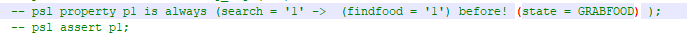
\includegraphics[scale=0.6]{PSL/preuveCode.PNG}
\caption{Assertion P1 révisé }
\end{figure} 

et obtenir le chronograme suivant :

\begin{figure}[!h]
\centering
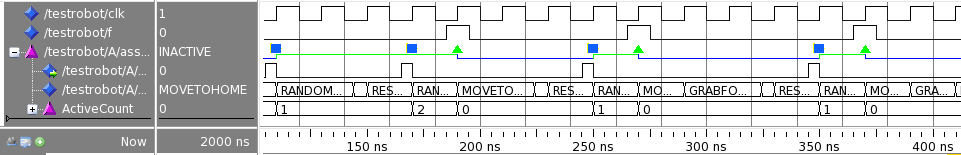
\includegraphics[scale=0.5]{PSL/preuve.PNG}
\caption{Assertion  de P1 révisé sur le chronograme }
\end{figure}

Même si au final notre formule était juste (P1 était un sous enssemble de notre assertion). Le code a état corrigé.

On peux faire de même avec P2 tel que :

\begin{figure}[!h]
\advance\leftskip+0cm
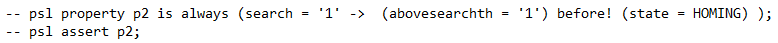
\includegraphics[scale=0.6]{PSL/P2P.PNG}
\caption{Assertion P2 révisé }
\end{figure} 



\newpage
\section{Annexes}
\subsection{Différences de code entre la partie 1 et 2 du projet}

Dans count.vhd, le test pour le branchement avec la détection du start devais ce fait avant celui du front montant 
\begin{figure}[!h]
\advance\leftskip+0cm
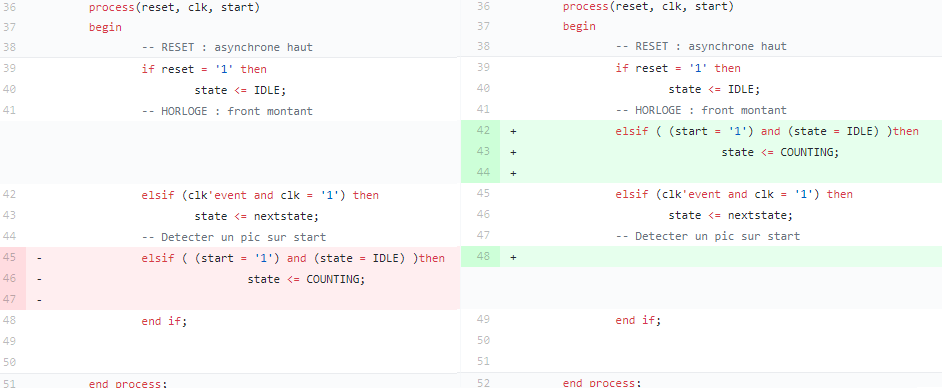
\includegraphics[scale=0.6]{modifCount.PNG}
\caption{Différence avec la première partie du projet de count.vhd}
\end{figure} 

Très peu de modification du testbench du robot
\begin{figure}[!h]
\centering
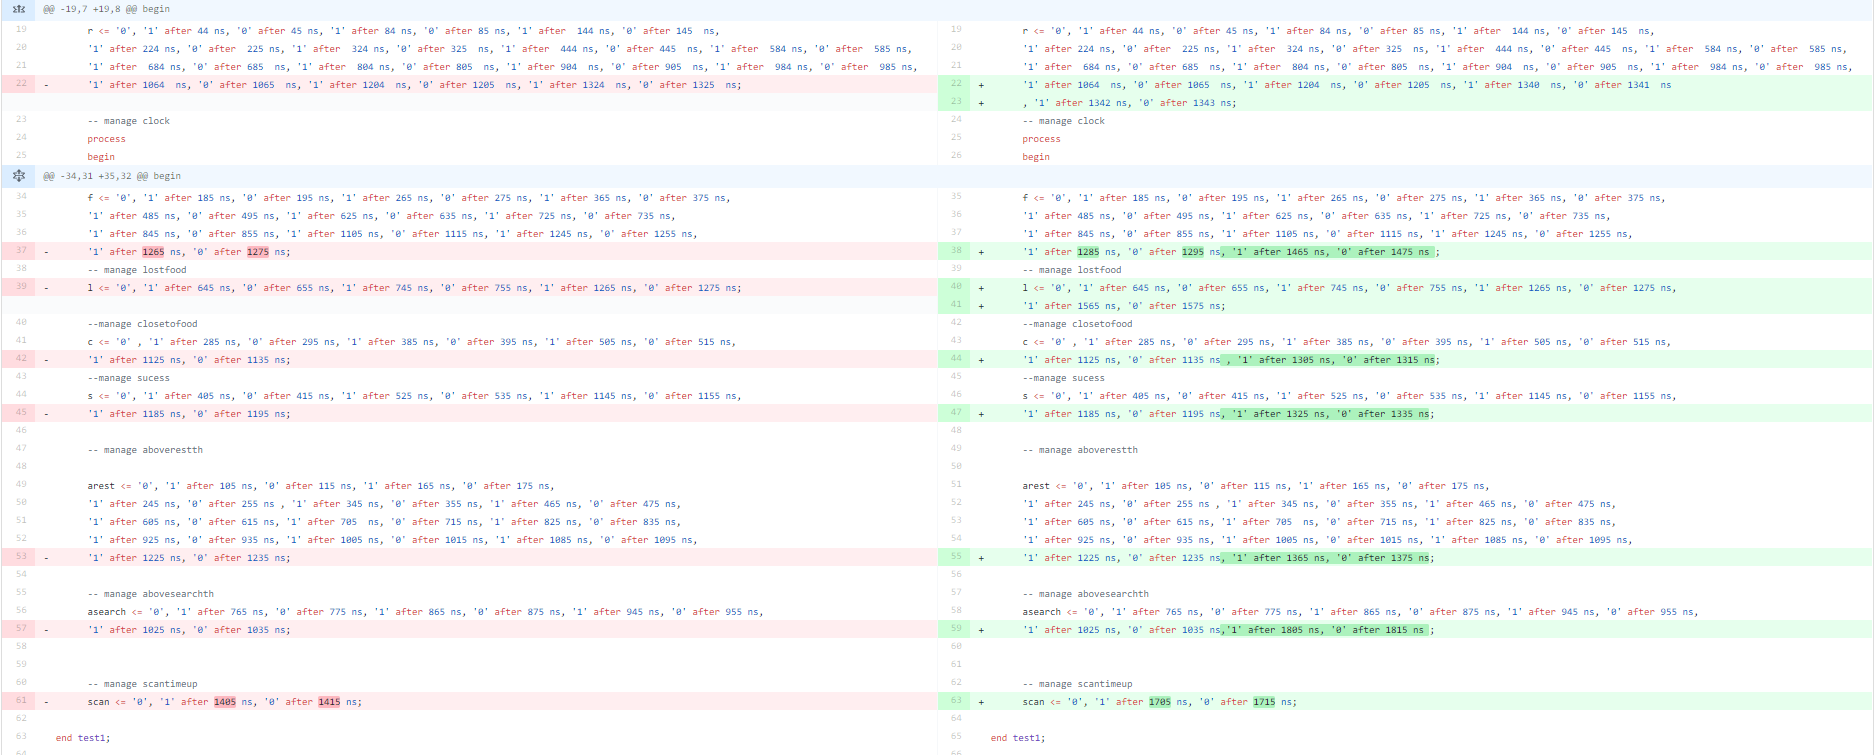
\includegraphics[scale=0.5]{changeR.PNG}
\caption{Différence avec la première partie du projet de testRobot.vhd }
\end{figure}

Dans robot.vhd, seul les PSL property ont était ajouté. J'ai aussi modifié le elsif par des else (voir dans les annexes suivantes).
\sautligne

Le testbench du système n'as pas était touché.
\sautligne

Le code est disponible sur : \url{https://github.com/egobiah/ARC}

\newgeometry{left=1cm,bottom=+2.5cm}
\begin{landscape}


\subsection{Le compteur}
\begin{figure}[!h]
\centering
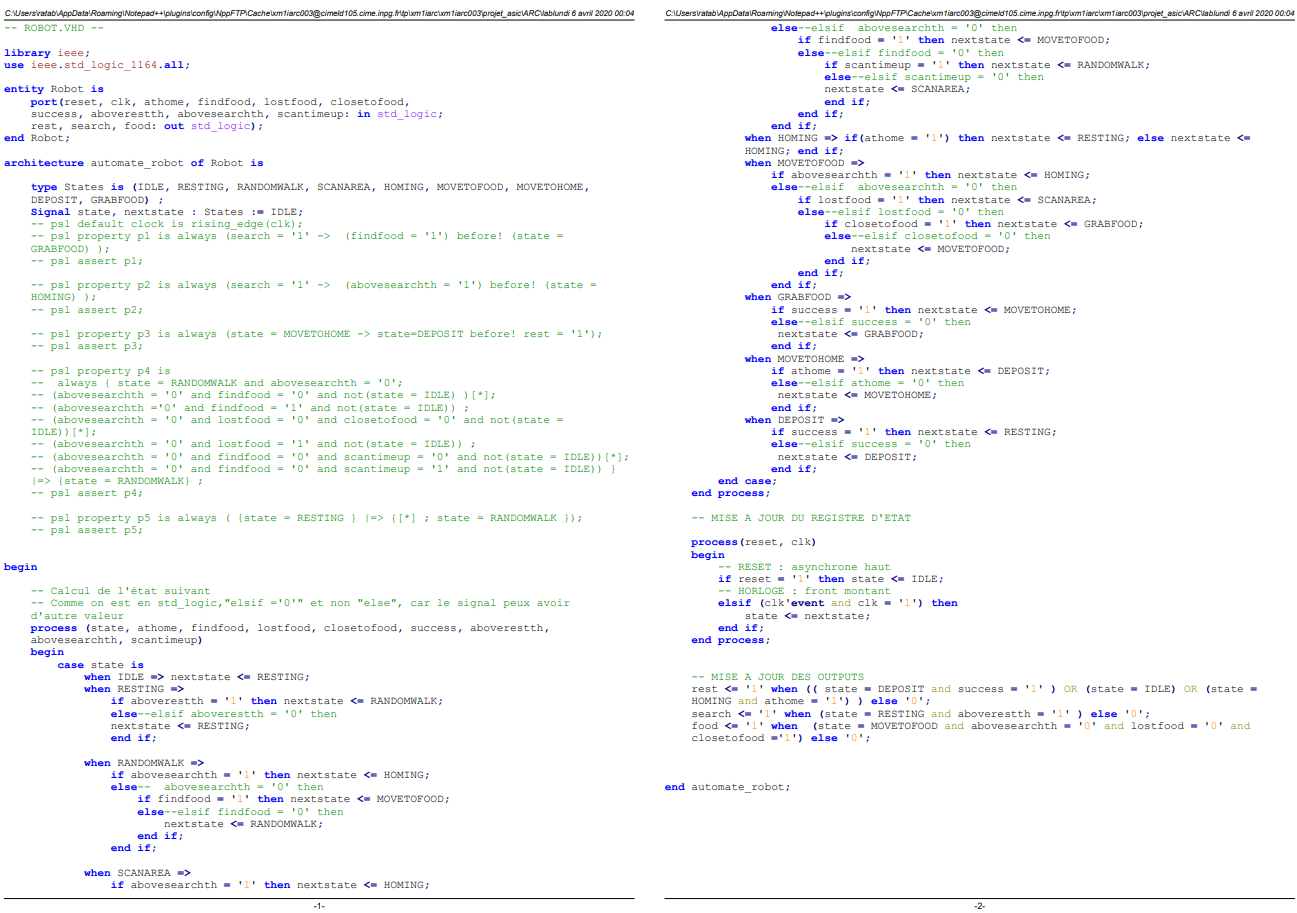
\includegraphics[scale=0.60]{robot.PNG}
\caption{count.vhd}
\end{figure} 

\newpage

\subsection{Architecture du robot}
\begin{figure}[!h]
\centering

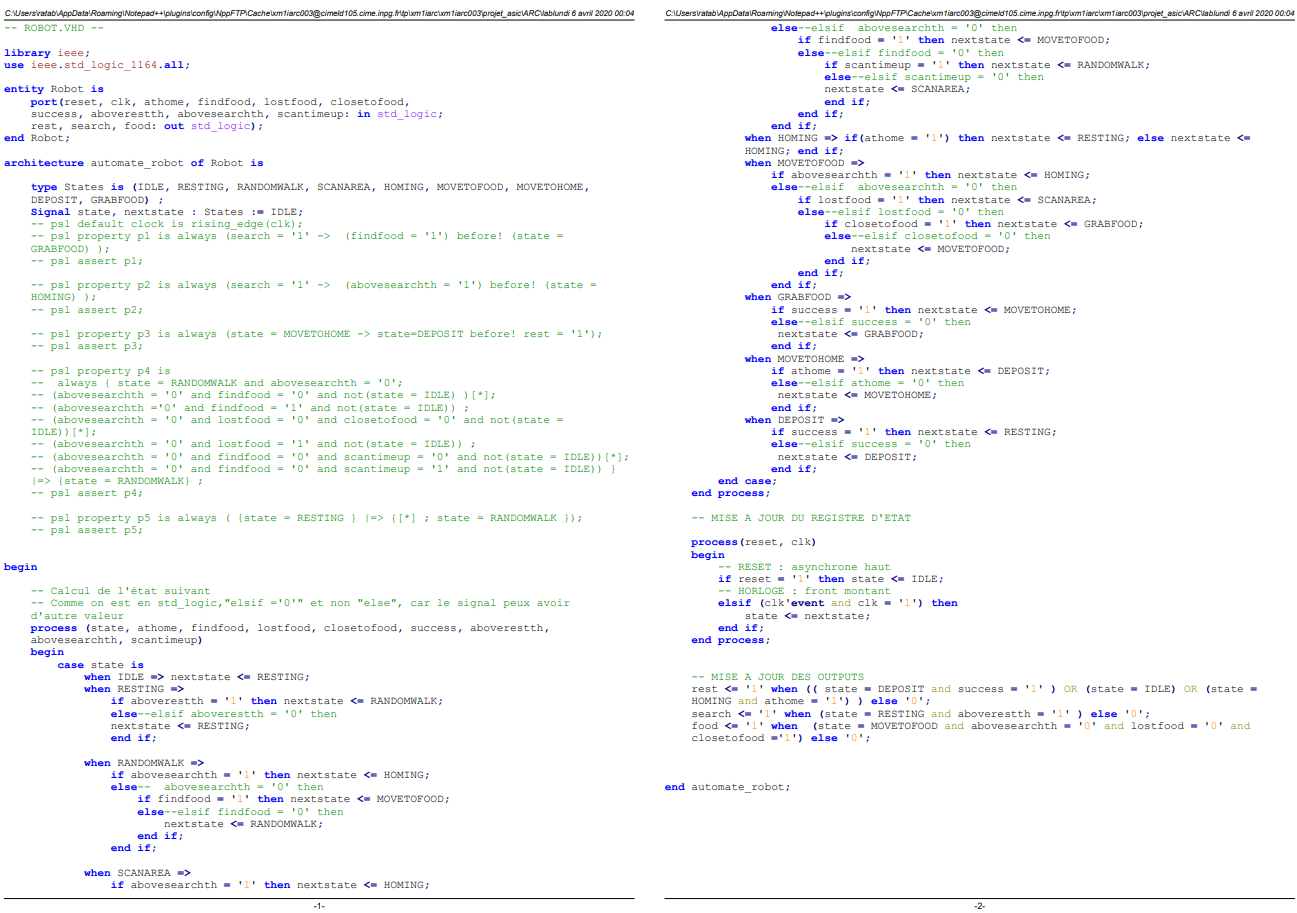
\includegraphics[scale=0.60]{robot.PNG}
\caption{robot.vhd}
\end{figure} 

\newpage

\subsection{TestBench du robot}
\begin{figure}[!h]
\centering

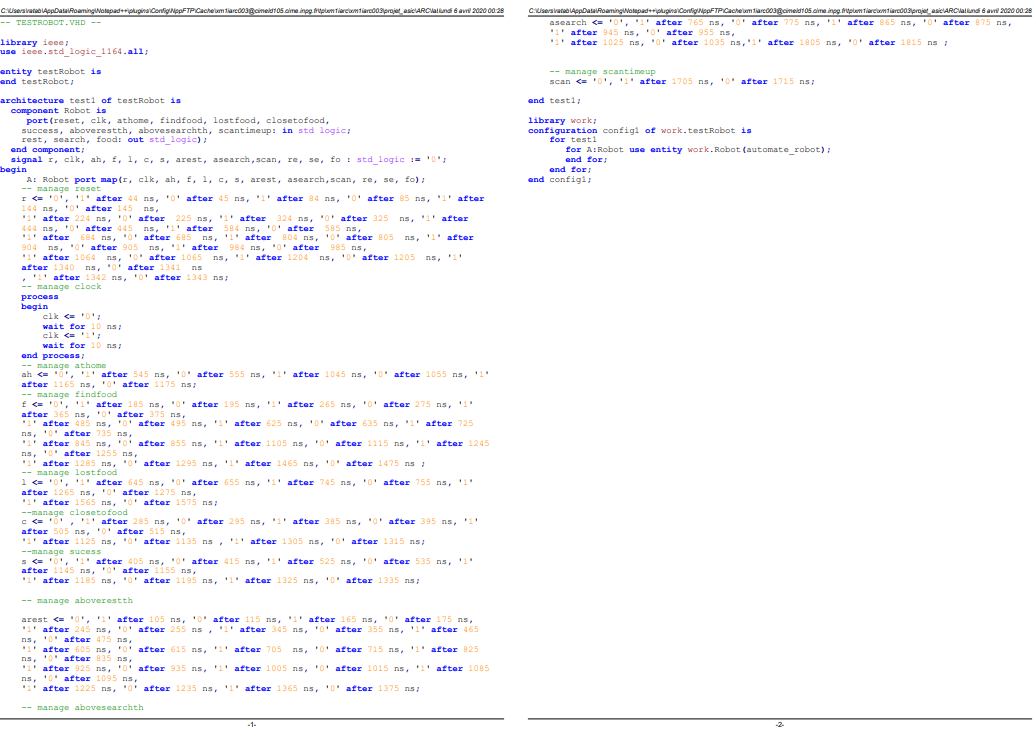
\includegraphics[scale=0.75]{testrobot.PNG}
\caption{testRobot.vhd}
\end{figure} 

\newpage

\subsection{TestBench du système}
\begin{figure}[!h]
\centering

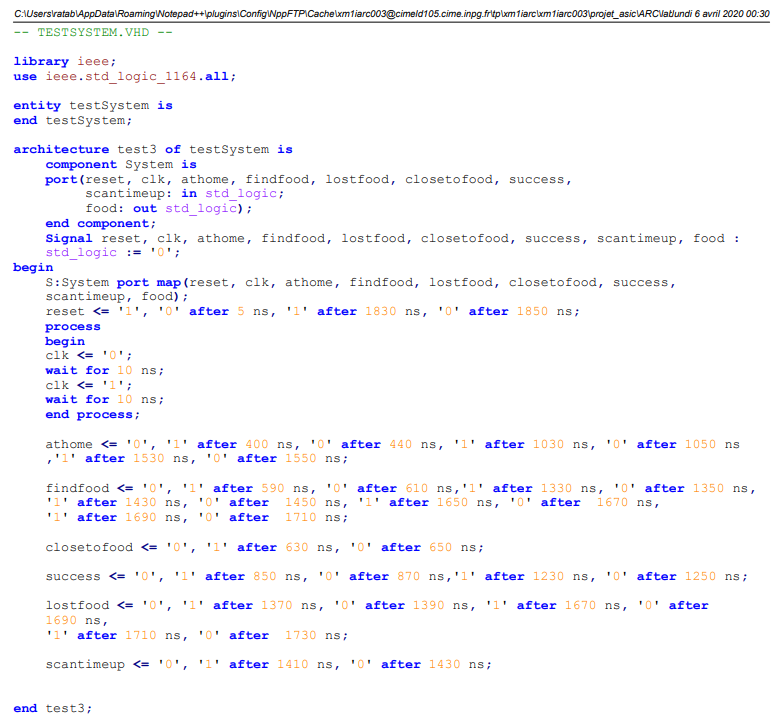
\includegraphics[scale=0.78]{testSystem.PNG}
\caption{testSystem.vhd}
\end{figure} 






\restoregeometry
\end{landscape}

\end{document}